\documentclass[12pt]{article}
\special{papersize=210mm,297mm}
\usepackage[top=1.5cm,bottom=1.5cm,left=2cm,right=2cm]{geometry}
\usepackage[skip=12pt plus1pt, indent=0pt]{parskip}

% Usual packages
\usepackage{graphicx}
\usepackage{hyperref}

\usepackage{fancyhdr}
\usepackage{amsmath}
\usepackage{cancel}
\usepackage{amssymb}
\usepackage{eurosym}
\usepackage{multicol}
\usepackage{rotate}
\usepackage{tabularx}
\usepackage{floatrow}
\usepackage{color}
\usepackage{colortbl}
\usepackage{braket}
\usepackage[shortcuts]{extdash}
\setlength{\headheight}{15.2pt}
\pagestyle{fancy}
\renewcommand{\headrulewidth}{0.5pt}
\renewcommand{\footrulewidth}{0.5pt}

\fancyhf{}
%%%% colors
\definecolor{orange}{RGB}{250,167,12}
\definecolor{yellow}{RGB}{246,250,12}
\definecolor{green}{RGB}{128,238,1}
\definecolor{green2}{RGB}{0,250,154}
\definecolor{black}{RGB}{0,0,0}
\definecolor{blue}{RGB}{0,0,255}
\definecolor{red}{RGB}{255,0,0}
\definecolor{white}{RGB}{255,255,255}
\definecolor{burlywood1}{RGB}{255,211,155}
\definecolor{chocolate1}{RGB}{255,127,36}
\definecolor{sepia}{RGB}{94,38,18}
\newcommand{\blue}[1]{\textcolor{blue}{#1}}
\newcommand{\sepia}[1]{\textcolor{sepia}{#1}}
\newcommand{\red}[1]{\textcolor{red}{#1}}
\newcommand{\green}[1]{\textcolor{green}{#1}}
\newcommand{\yellow}[1]{\textcolor{yellow}{#1}}
\newcommand{\orange}[1]{\textcolor{orange}{#1}}
%%%% mathematical definitions
\DeclareMathOperator{\Tr}{Tr}
\def\npab{\noindent \textbullet ~}
\def\npa{\noindent}
\def\npat{\noindent \textcolor{blue}{$\blacktriangleright$} ~}
\def\npac{\noindent $\circledast$ ~}
\def\nn{{\bf \nabla}}
\def\df{{\rm d}}
\def\cro{\times}
\def\ip{i^{'}}
\def\jp{j^{'}}
\def\kp{k^{'}}
\def\deg{$^{\circ}$}
\def\rhoc{\textcolor{red}{\rho}}
\def\uic{\textcolor{red}{u_i}}
\def\ujc{\textcolor{red}{u_j}}
\def\pgc{\textcolor{red}{P_{\rm g}}}
\newcommand{\ve}[1]{{\rm\bf {#1}}}
\def\ez{\ve{e}_z}
\def\ey{\ve{e}_y}
\def\ex{\ve{e}_x}
\def\ezero{\ve{e}_{0}}
\def\eplu{\ve{e}_{+1}}
\def\emin{\ve{e}_{-1}}
\def\definition{:=^{\!\!\!\!\!\!\!\textrm{def}}}
\newcommand{\bg}[1]{{\boldsymbol {#1}}}
\newcommand*\tavg[1]{%
  \hbox{%
    \vbox{%
      \hrule height 0.5pt % The actual bar
      \kern0.5ex%         % Distance between bar and symbol
      \hbox{%
        \kern-0.1em%      % Shortening on the left side
        \ensuremath{#1}%
        \kern-0.1em%      % Shortening on the right side
      }%
    }%
  }%
}
\title{Theoretical Astrophysics: Physics of Sun and Stars\\
Homework 1 - solutions}
\author{P. K\"{a}pyl\"{a}, I. Mili\'{c}}
\date{\today}
%%%%
\begin{document}
\maketitle

\textbf{Deadline for this homework is 14/05 23:59}



{\bf Problem 1:} Following the exercise we did at the introductory hands-on, where we created our own Herzschprung-Russel (HR) diagram, calculate the radii of the stars in the database, assuming a star is radiating like blackbodies of the temperature equal to the effective temperature of the star. The file and the meaning of its contents can be found in the hands-on notebook.

For this you will have to: 
\begin{enumerate}
  \item Transform the absolute magnitude of the star to its luminosity. For that you can use: 
\begin{equation}
  M - M_{\odot} = 2.5\log \frac{L_{\odot}}{L}
\end{equation}
  where $M_{\odot} = 4.83$ is the absolute magnitude of the Sun. 

  \item Transform the stars \emph{color index} into the temperature. For this, wikipedia as an excellent article that we suggest having a look at \href{https://en.wikipedia.org/wiki/Color_index}{here}.

\end{enumerate}

\textbf{Solution:} The solution is given the accompanying notebook,
and here we provide a few comments regarding what is actually going
on. First, the quantities that are obtained from the txt file are the
relative magnitude (aka apparent brightness) of the star, $B-V$ color
index, and, finally, the paralax of the star. Few sentences on each of
those:

Relative magnitude of the star is the quantity that describes how
bright the stars seem. The relative magnitude $m$ is defined with
respect to Vega, which is a bright star in the constellation Lyrae:
\begin{equation}
m - m_{\rm Vega} = 2.5 \log \frac{\mathcal{E}_{\rm Vega}}{\mathcal{E}}
\end{equation}
where $\mathcal{E}$ is, in this case, the so called ``irradiance" or
the recieved flux density from the star and it is related to the
luminosity of star as:
\begin{equation}
\mathcal{E} = \frac{L}{4\pi d^2},
\end{equation}
where $L$ is the luminosity and $d$ is the distance to the star.

Now, we are obviously interested in absolute measurements, i.e., we
want to remove the distance from the game. So we define the absolute
magnitude, which is the relative magnitude the star would have if it
was 10 parsecs away from us. It turns out, then:
\begin{equation}
M = m + 5 - 5 \log d,
\end{equation}
which means that for the stars of fixed $m$, those that are further,
are actually brigther (recall that smaller $M$ means brighter star!).

Finally, it turns out that the distance to the star is inverse of its
parallax. So, we can easily calculate $d$ and use it to find $M$. From
$M$, it is easy to find $L$, by comparing the star to the Sun:
\begin{equation}
M - M_{\odot} = 2.5 \log \left(\frac{L_{\odot}}{L}\right).
\end{equation}
If we recall that the luminosity of the star can be related to it's
``surface'' temperature (actually it's the effective temperature,
because star does not actually have a surface, but more about that in
a couple of weeks):
\begin{equation}
L = 4\pi R^2 \sigma T_{\rm eff}^4,
\end{equation}
we realize that we miss the temperature. Temperature can be estimated
from the color of the star (does this make sense? maybe discuss for a
couple of minutes?). The observational measure of the color is the so
called B-V color index. It is a difference of magnitudes made in
different filters that transmit a different range of colors. We can
estimate the effective temperature from the color index like this:
\begin{equation}
T = 4600 \left ( \frac{1}{0.92 (B-V) + 1.7} + \frac{1}{0.92 (B-V) +
  0.62} \right ){\rm K}.
\end{equation}
Now, we have all the quantities to calculate the radius (Have a look
at the notebook).

The values range from few 1000s of kms to tens of millions of
kms. What do you make of that? Can you somehow cluster stars according
to their radii?

\pagebreak

{\bf Problem 2:} For a gas in hydrostatic equilibrium with a constant
mean molecular mass and constant temperature, in a constant
gravitational field, show that the pressure falls off exponentially
with height:
\begin{equation}
p = p_0 e^{-z/H}
\end{equation}
where $H$ is the so-called scale height. Find the expression for the
scale height and calculate its value for the Earth's atmosphere and
the solar atmosphere (for the moment, assume the Sun is composed of
pure neutral hydrogen atoms, for simplicity you can assume that
Earth's atmosphere is composed of pure Nitrogen).

{\bf Solution:} Starting from the equation of hydrostatistic
equilibrium for a spherical body:
\begin{equation}
\frac{dp(r)}{dr} = - \rho(r) G\frac{M(r)}{r^2},
\end{equation}
we will assume that we are at the surface and that we are expressing
things in term of height $z$, and that the gravitational acceleration
is constant as $z\ll R$ and $M(z) = M(R)$. We then have:
\begin{equation}
\frac{dp}{dz} = - \rho(z) g. 
\end{equation}
Then, we know that $p = nkT$ and that $\rho = n \mu$ where $\mu$ is
the mean molecular mass. We then get $\rho = p \mu/ (kT)$. Our
equation becomes:
\begin{equation}
\frac{dp}{dz} = - \frac{p \mu}{kT} g,
\end{equation}
which translates to:
\begin{equation}
\frac{dp}{p} = - \frac{\mu g}{kT} dz,
\end{equation}
which after solving and imposing limits turns into: 
\begin{equation}
\ln p |_{p_0}^p = - \frac{g \mu}{kT} z|_0^z.
\end{equation}
Therefore:
\begin{equation}
p(z) = p(0) e^{-z/H},
\end{equation}
where $H = kT / \mu g$.

\emph{Discuss the result a bit. Does it make sense how $H$ scales with
temperature, composition, surface gravity...}

For Earth, we will use $T = 300 K$, $g=9.81 {\rm m/s^2}$, and $\mu=28
m_u$ (this is for two Nitrogens) where $m_u$ is the atomic mass
unit. We should get something like 8 km. So density of air at Mount
Everest is 2.73 times smaller than here!

For the Sun, we can use $T = 6000$\,K. $g = 274 {\rm m/s^2}$, and
$\mu=1 m_u$ (neutral hydrogen), that leads us to roughly
200\,km. Interestingly this height scale is related to the size of the
granules at the solar surface (see the picture below).

\begin{figure}
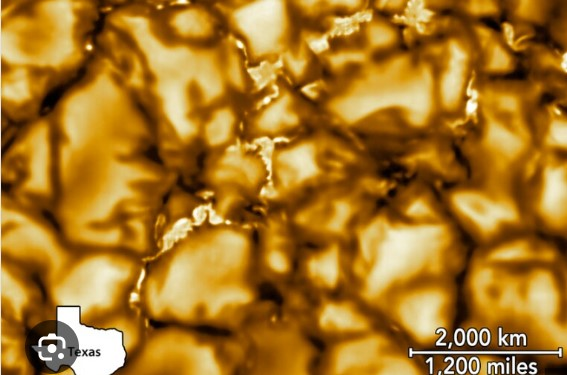
\includegraphics[width=0.6\textwidth]{granulation.jpg}
\caption{Granules observed by DKIST solar telescope. Credit: AURA/NSF/DKIST/NSO}
\end{figure}

\pagebreak

{\bf Problem 3:} Stefan-Boltzmann law describes the emergent flux from
a blackbody. That is, total energy per unit surface in unit time,
emitted into the $2\pi$ solid angle (full sphere is $4\pi$ but we are
only looking at the outgoing half).

Planck law describes the intensity of radiation in a blackbody,
intensity is defined as:
\begin{equation}
I_\lambda = \frac{dE}{dt dS d\Omega d\lambda \cos \theta},
\end{equation}
where $\Omega$ is the solid angle $d\Omega = \sin \theta d\theta
d\phi$, and $\theta$ and $\phi$ describe the direction of propagation
of radiation. For Planck's law:
\begin{equation}
I_\lambda = \frac{2hc^2}{\lambda^5} \frac{1}{e^{hc/\lambda k T} - 1}.
\end{equation}

Using the Planck's law, derive Stefan-Boltzmann law:
\begin{equation}
F = \frac{dE}{dt dS} = \sigma T^4.
\end{equation}

{\bf Solution:} A photon impinging surface $dS$ under the angle
$\theta$ will transport the energy $E \cos \theta$ through the
surface. So, to get the total energy transported through the surface
per unit time, we need to integrate the intensity, times $\cos \theta$
over all the possible impinging angles.
\begin{equation}
F_\lambda = \int_{\theta=0}^{\pi} \int_{\phi=0}^{2\pi} I(\theta, \phi) \cos \theta \sin \theta d \phi d \theta.
\end{equation}
This will, however, turn into zero! What did we do wrong? Well, we
considered \emph{all} the directions. We got zero. That makes sense,
as the Planck's law describes a body in the state of thermal
equilibrium so, flux has to be zero in order to keep the body in
equilibrium.

We treat stars as bodies where equlibrium holds locally, but the flux
is still transported due to very small gradients. Light lost at the
surface is replenished by the energy coming from below.

So, at the surface of the star we have a paradoxical situation: the
photons coming from under the surface are approximated by the
blackbody at the surface temperature, and there are no photons coming
from above. Then we will get the following for the outgoing flux:
\begin{equation}
F_\lambda = \int_{\theta=0}^{\pi/2} \int_{\phi=0}^{2\pi} I(\theta, \phi) \cos \theta \sin \theta d \phi d \theta.
\end{equation}
Noticing that the radiation is isotropic and using $\cos \theta = \mu$
(not the same $\mu$ as in the previous problem!!!!), we should get
that:
\begin{equation}
F_\lambda = \pi I_\lambda.
\end{equation}

Now, we need the total flux, over all frequencies / wavelengths. So:
\begin{equation}
F_\lambda = \int_0^{\infty} \frac{2 \pi hc^2}{\lambda^5} \frac{d\lambda}{e^{hc/\lambda k T} - 1},
\end{equation}
which, by using $x = hc/\lambda k T$ and using Wolfram alpha or
similar, should give us Stefan Boltzmann law!

\begin{figure}
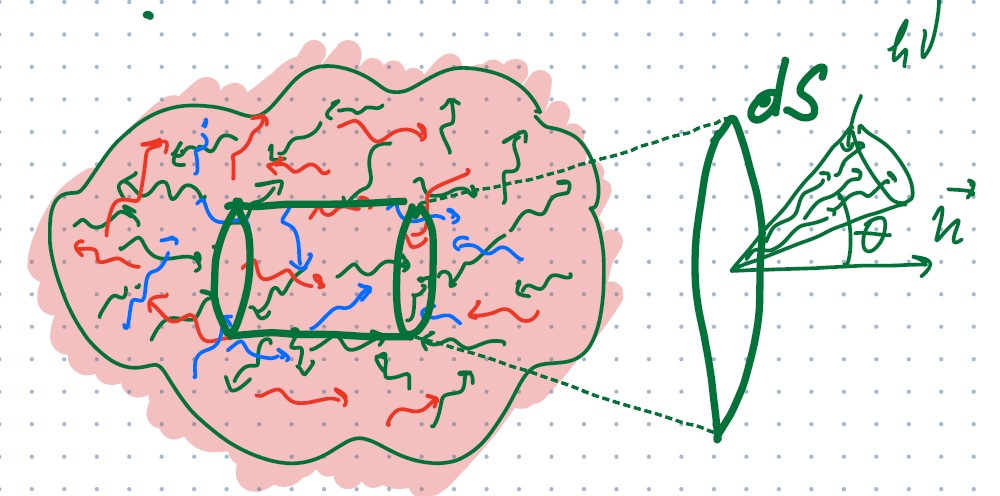
\includegraphics[width=0.6\textwidth]{flux.jpg}
\caption{Flux}
\end{figure}

 
{\bf Useful physical constants}
\begin{itemize}
  \item $R_{\odot} = 696 \times 10^6\,{\rm m}$
  \item $m_{\odot} = 1.989 \times 10^{30}\,{\rm kg}$
  \item $L_{\odot} = 3.83 \times 10^{26}$~W
  \item $T^{\rm eff}_{\odot} = 5777\,{\rm K}$
  \item $1\,{\rm AU} = 1.496 \times 10^8\,{\rm km}$
  \item $c = 2.997 \times 10^8\,{\rm m/s}$
  \item $G = 6.674 \times 10^{-11}$~Nm$^2$/kg$^2$
  \item $k = 1.38\cdot10^{-23}$~J/K
  \item $m_{\rm H} = 1.67\cdot10^{-27}$~kg
  \item $h=6.626 \times 10^{-34}$~J~s.
  \item $k=1.38 \times 10^{-23}$~J/K.
  \item $\sigma=5.67 \times 10^{-8}$~W/m$^2$ K$^4$.
\end{itemize}
\end{document}
